\fontfamily{\sfdefault}\selectfont
% XCircuit output "tdc_quant.tex" for LaTeX input from tdc_quant.ps
\def\putbox#1#2#3#4{\makebox[0.00000in][l]{\makebox[#1][l]{}\raisebox{\baselineskip}[0.00000in][0.00000in]{\raisebox{#2}[0.00000in][0.00000in]{\scalebox{#3}{#4}}}}}
\def\rightbox#1{\makebox[0.00000in][r]{#1}}
\def\centbox#1{\makebox[0.00000in]{#1}}
\def\topbox#1{\raisebox{-0.60\baselineskip}[0.00000in][0.00000in]{#1}}
\def\midbox#1{\raisebox{-0.20\baselineskip}[0.00000in][0.00000in]{#1}}
   \scalebox{1}{
   \normalsize
   \parbox{3.50000in}{
   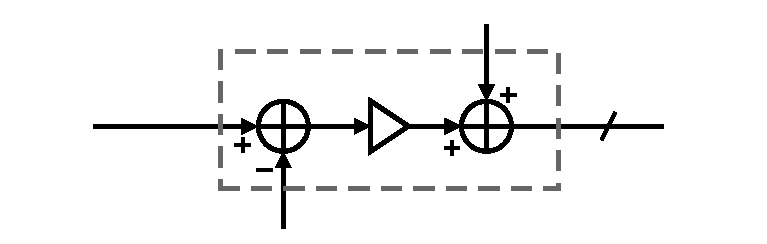
\includegraphics[scale=0.70000]{./figs/tdc_quant.pdf}\\
   % translate x=432 y=396 scale 0.38
   \putbox{0.46200in}{0.63700in}{1.20}{$\Phi_{ref}$[n]}%
   \putbox{1.35100in}{0.08400in}{1.20}{$\Phi_{div}$[n]}%
   \putbox{2.68100in}{0.66500in}{1.20}{e$_\Phi$[n]}%
   \putbox{1.77800in}{0.70700in}{1.20}{\rotatebox{-360}{$\frac{\mathrm{M}}{2\pi}$}}%
   \putbox{1.47000in}{0.63700in}{1.20}{$\Phi_e$}%
   \putbox{2.31700in}{0.97300in}{1.20}{q$_{TDC}$[n]}%
   \putbox{1.02900in}{0.95900in}{1.20}{TDC}%
   } % close 'parbox'
   } % close 'scalebox'
   \vspace{-\baselineskip} % this is not necessary, but looks better
\fontfamily{\rmdefault}\selectfont
